\documentclass[twoside]{AiTeX}



\title{PEV}
\author{A.L.K.}
\date{Diciembre 2021}
\begin{document}
%\datos{facultad}{universidad}{grado}{asignatura}{subtitulo}{autor}{curso}
\datos{Informática}{Universidad Complutense de Madrid}{Ingeniería informática}{Programación Evolutiva}{Memoria de la práctica 3}{Alejandro Barrachina Argudo \\ Adrià Carreras Bagur }{2023}
\portadaApuntes
\pagestyle{empty}
\tableofcontents
\pagestyle{empty}
\justify
\pagestyle{fancy}

\newpage

\chapterA{Capturas de funcionamiento}

\begin{figure}[H]
    \centering
    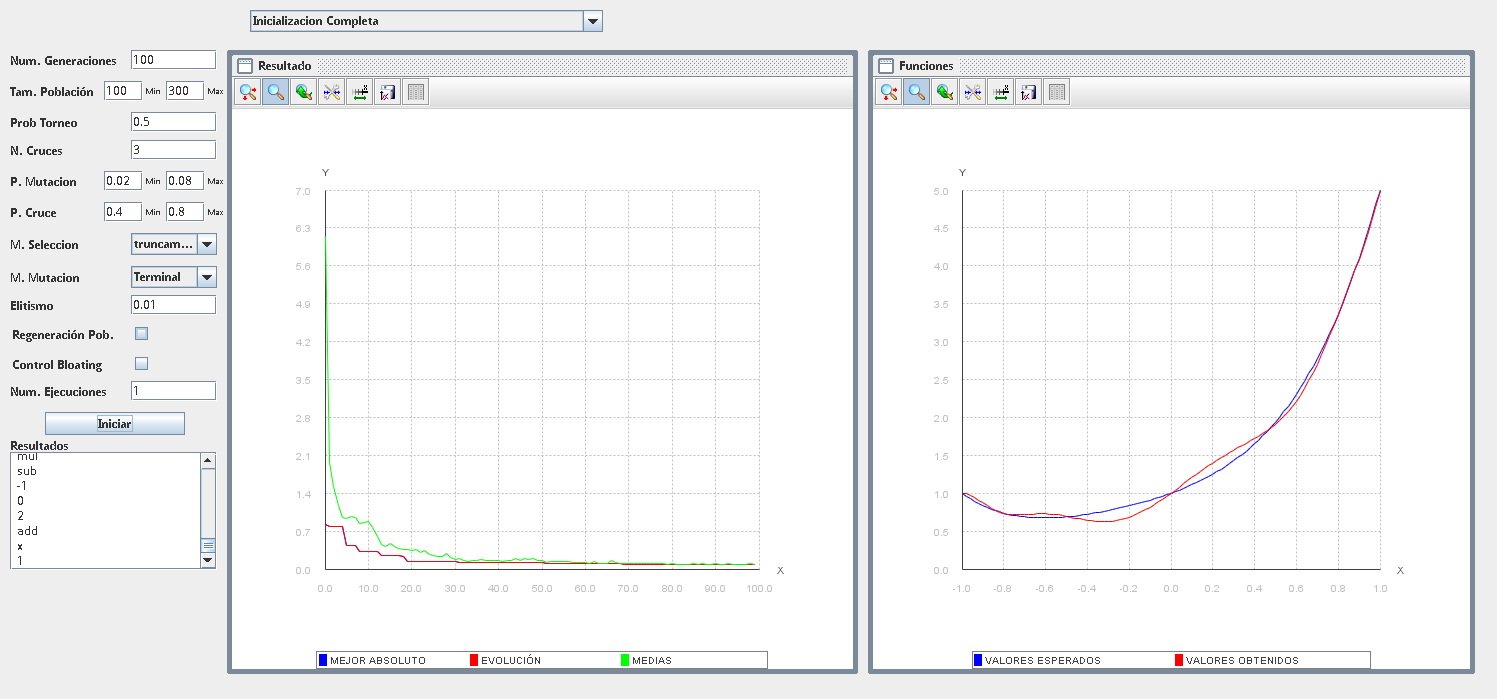
\includegraphics[width = \textwidth]{Images/Captura1.png}
    \caption{Captura 1}
    \label{fig:1}
\end{figure}



\begin{figure}[H]
    \centering
    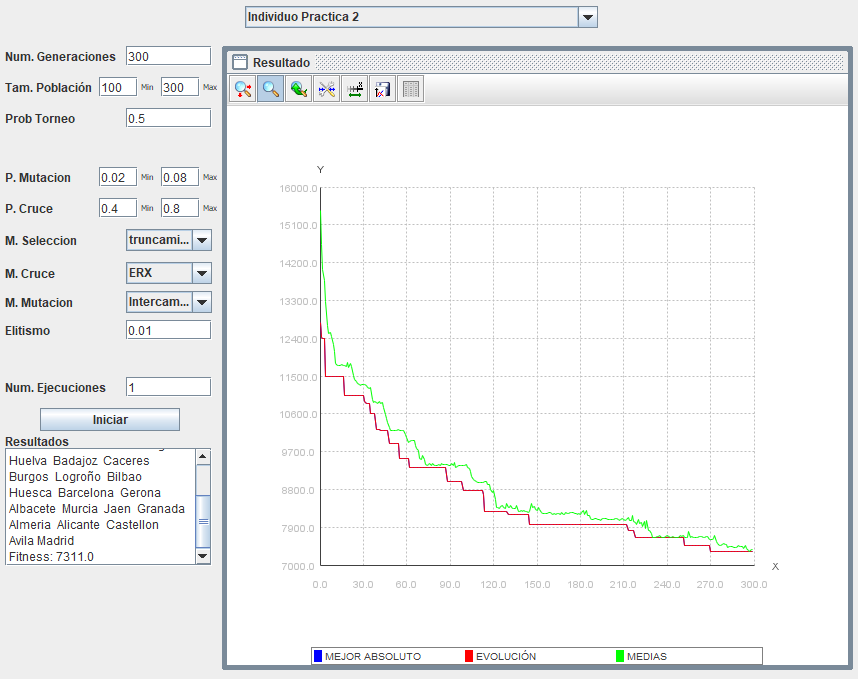
\includegraphics[width = \textwidth]{Images/Captura2.png}
    \caption{Captura 2}
    \label{fig:2}
\end{figure}



\begin{figure}[H]
    \centering
    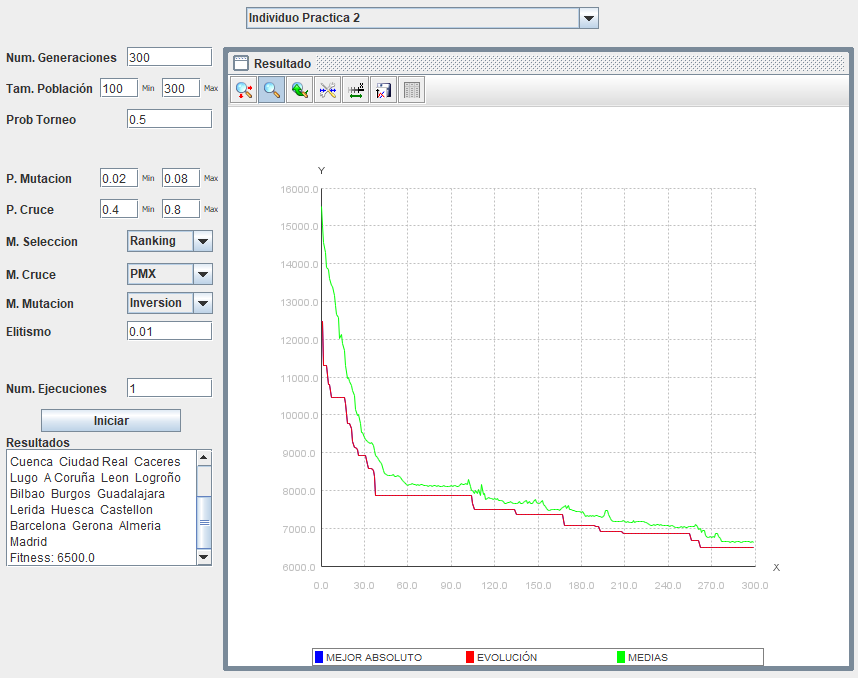
\includegraphics[width = \textwidth]{Images/Captura3.png}
    \caption{Captura 3}
    \label{fig:3}
\end{figure}



\chapterA{Observaciones de la práctica, arquitectura del código y ejecución}

\section{Observaciones}

Se han imnplementado los 2 tipos de inicializaciones distintas dentro de los árboles y Ramped and Half que combina las dos, dando muy buenos resultados.

Para el control de bloating se ha cambiado al cruce básico para que se hagan diferentes ejecuciones y así poder descartar individuos que empeorarían el fitness. Para evitar estre cruce destructivo se ha añadido a la GUI el apartado Numero de Cruces, aunque hay que tener en cuenta que aumentarlo demasiado podría empeorar el tiempo de ejecución.
Además para el bloating se ha utilizado el método de la penalización.

Las mutaciones Terminales y Funcionales son muy eficientes aunque pueden llevar a una convergencia prematura si no se utilizan adecuadamente.
Las mutaciones de SubArbol y Expansion dan resultados muy buenos, pero si se utilizan demasiado o sin control de bloating podrían hacer que la ejecución tarde más.
La mutación de Permutación es un punto medio, no alarga tanto los árboles y consigue buenas soluciones.

Se añadió la Regeneración de Población para momentos en los que los árboles pudieran quedarse atascados en resultados no óptimos, esta opción se puede elegir desde la GUI

Los métodos de selección que nos han dado mejores resultados como ya hemos visto en otras prácticas han sido el truncamiento y el ranking, siendo el truncamiento en esta practica mucho más eficiente.

\section{Arquitectura}

Para mantener todo el código organizado, se usa la siguiente estructura de paquetes:

\begin{itemize}
    \item\textbf{go2:} paquete que engloba toda la práctica.
    \item\textbf{g02.cruces:} Paquete que reúne el único cruce de esta prática bajo la interfaz Cruces.
    \item\textbf{g02.individual:} Paquete que contiene el individuo de la práctica 3 bajo la clase padre Individuo<T>.
    \item\textbf{g02.Selections}: Paquete para reunir las distintas selecciones usadas en la práctica bajo la clase padre Selection<T>.
    \item\textbf{g02.Ventana}: Paquete para la interfaz gráfica de la práctica y el método main.
\end{itemize}

Para una visión mas completa del proyecto, desde el navegador puede abrir el archivo G02/target/site/index.html

\section{Ejecución y compilación de la práctica}

Al ser un proyecto en maven se puede importar directamente desde eclipse con la opción de abrir proyectos del sistema de archivos.

Para compilar el proyecto solo hay que darle al botón de \textit{run} y debería instalar las dependencias necesarias. Si no fuera así se puede ejecutar el comando \textit{mvn install} para instalar todas las dependencias.

Así mismo, el proyecto se puede correr desde el propio eclipse usando el botón de \textit{run}, usando la configuración de \textit{aplicación java} y como clase principal g02.Ventana.ventana.

El archivo jar se encuentra en la carpeta P03/target/


\chapterA{Distribución de trabajo y conclusiones}

\section{Distribución}

Adrià ha hecho la GUI añadiendo las variables que se pueden manejar y el nuevo gráfico que compara la solución obtenida con la esperada; los métodos de mutación y ha trabajado con las clases del Árbol y el Cromosoma.

Alejandro ha hecho la implementación del cruce de la práctica 3, la regeneración de la población, el control de bloating y también ha trabajado con las clases de Árbol e Individuo.

\section{Conclusiones}

Nos hemos dado cuenta de que para solucionar este problema hay que tener muy en cuenta la optimización del código en general, los árboles pueden llegar a ser muy costosos y hay que minimizar los individuos que no vayan a aportar a la solucion.

Los métodos de selección que mejores resultados nos han dado han sido: Truncamiento y Ranking, siendo el Truncamiento el más efectivo, aunque más propenso a quedarse estancado.

Las mutaciones han sido muy útiles y pueden afectar mucho al resultado, cada una tiene su función y se utiliza de una manera distinta, aunque la Permutación ha dado muy buenos resultados.

El control del Bloating es esencial en este problema.

\end{document}
